\documentclass[12pt,a4paper]{article}

\usepackage[utf8]{inputenc}
\usepackage[T1]{fontenc}
\usepackage[spanish]{babel}
\usepackage{amsmath,amssymb}
\usepackage{graphicx}
\usepackage{booktabs}
\usepackage{hyperref}
\usepackage{geometry}
\usepackage{listings}
\usepackage{xcolor}
\usepackage{float}

\geometry{margin=2.5cm}

\lstset{
    basicstyle=\ttfamily\small,
    breaklines=true,
    frame=single,
    language=C++,
    showstringspaces=false,
}

\title{Tarea 2 — Introducción a la Computación Paralela\\
\large Procesamiento de Imágenes en CUDA:\\
Cálculo de la Matriz de Covarianza}
\author{Cecilia Hernández y Álvaro Guzmán}
\date{Junio 2026}

\begin{document}

\maketitle

%---------------------------------------------------------------------
\section{Introducción}
%---------------------------------------------------------------------

El objetivo de esta tarea es implementar, analizar y optimizar el procesamiento
masivo de un volumen de imágenes a color utilizando CUDA. Específicamente, se
calcula la matriz de covarianza del conjunto de imágenes centradas, lo cual
constituye una operación de álgebra lineal densa de alta demanda computacional
y de memoria.

\subsection{Formalización matemática}

Dado un conjunto de $m$ imágenes, donde cada imagen aplanada es un vector
$\mathbf{v}^{(k)} \in \mathbb{R}^n$ con $n = \text{ancho} \times \text{alto}$:

\begin{enumerate}
    \item \textbf{Vector promedio:}
        $\boldsymbol{\mu} = \frac{1}{m}\sum_{k=0}^{m-1} \mathbf{v}^{(k)}$
    \item \textbf{Matriz centrada:}
        $\bar{\mathbf{v}}^{(k)} = \mathbf{v}^{(k)} - \boldsymbol{\mu}$
    \item \textbf{Matriz de covarianza:}
        $\mathbf{C} = \frac{1}{m}\sum_{k=0}^{m-1}
         \bar{\mathbf{v}}^{(k)} \cdot (\bar{\mathbf{v}}^{(k)})^T$
\end{enumerate}

El resultado $\mathbf{C} \in \mathbb{R}^{n \times n}$ es una matriz simétrica
y semidefinida positiva.

%---------------------------------------------------------------------
\section{Entorno de ejecución}
%---------------------------------------------------------------------

\begin{table}[H]
\centering
\begin{tabular}{ll}
\toprule
Componente & Especificación \\
\midrule
CPU & \texttt{...} \\
GPU & NVIDIA GeForce RTX 3060 Laptop GPU \\
VRAM & 6144 MiB \\
Compute Capability & 8.6 (Ampere) \\
CUDA Toolkit & 11.2 \\
Host compiler & g++ 9.5.0 \\
Sistema operativo & Linux (Ubuntu 22.04) \\
\bottomrule
\end{tabular}
\caption{Entorno de ejecución}
\end{table}

%---------------------------------------------------------------------
\section{Diseño algorítmico}
%---------------------------------------------------------------------

\subsection{Fórmula incremental}

Para evitar dos pasadas sobre los datos (centrar y luego calcular covarianza),
se utiliza la identidad algebraica:

\begin{equation}
\mathbf{C} = \frac{1}{m}\sum_{k} \mathbf{v}^{(k)}(\mathbf{v}^{(k)})^T
            - \boldsymbol{\mu}\boldsymbol{\mu}^T
\end{equation}

Esto permite acumular $\sum \mathbf{v}$ y $\sum \mathbf{v}\mathbf{v}^T$ en una
sola pasada. Es particularmente útil para la versión con Streams, donde los
datos se procesan en batches independientes.

\subsection{Preprocesamiento}

Las imágenes del dataset DIV2K\_valid\_LR\_bicubic\_X4 tienen dimensiones
variables de aproximadamente $510 \times 340$ píxeles en RGB. Para obtener
vectores de dimensión uniforme $n$, se aplican los siguientes pasos:

\begin{enumerate}
    \item \textbf{Conversión a escala de grises:} usando
          \texttt{CImg::get\_RGBtoYCbCr().channel(0)} (luminancia).
    \item \textbf{Redimensionamiento a $32 \times 32$ píxeles:} mediante
          \texttt{CImg::resize()} con interpolación bilineal.
    \item \textbf{Aplanado y normalización:} cada imagen se aplana a un vector
          de $n = 1024$ elementos con valores en $[0, 1]$.
\end{enumerate}

\textbf{Dimensión elegida:} se seleccionó $n = 32 \times 32 = 1024 = 2^{10}$
siguiendo la recomendación del equipo docente. Con este tamaño, la matriz de
covarianza $\mathbf{C} \in \mathbb{R}^{1024 \times 1024}$ ocupa aproximadamente
4~MB en VRAM, dejando margen amplio para buffers adicionales. El parámetro
\texttt{--size} permite probar otras resoluciones (e.g., \texttt{--size 64}
para $n=4096=2^{12}$).

\textbf{Justificación de \texttt{resize} sobre \texttt{crop} o \texttt{pad}:}
DIV2K contiene imágenes de dimensiones variables. Un \texttt{crop} fijo de
$32 \times 32$ extraería menos del 1\% de cada imagen, descartando información
visual relevante. El \texttt{pad} introduciría regiones artificiales de ceros
que distorsionarían la covarianza. \texttt{CImg::resize()} con interpolación
bilineal preserva la escena completa y produce vectores de dimensión uniforme,
siendo la estrategia más adecuada para procesamiento masivo de imágenes.

El dataset completo se almacena en memoria paginada bloqueada
(\texttt{cudaMallocHost}) para permitir transferencias asíncronas en el
Experimento~2.

\subsection{Tiling en memoria compartida}

La matriz $\mathbf{C}$ de tamaño $n \times n$ se particiona en tiles de
$32 \times 32$. Cada bloque de $32 \times 32$ hilos computa un tile de $\mathbf{C}$,
iterando sobre el conjunto de imágenes. Para cada imagen, los hilos cargan
cooperativamente dos segmentos del vector a memoria compartida,
reduciendo los accesos a memoria global.

%---------------------------------------------------------------------
\section{Experimento 1: Implementación tradicional}
%---------------------------------------------------------------------

\subsection{Descripción}

Se asume que todo el dataset cabe en VRAM. Se utiliza el Stream 0 por defecto.
El pipeline es completamente síncrono:

\begin{enumerate}
    \item \texttt{cudaMemcpy} H$\rightarrow$D del dataset completo.
    \item Kernel \texttt{reduce\_mean}: reducción para obtener $\sum\mathbf{v}$.
    \item Kernel \texttt{cov\_accumulate\_tiled}: acumula $\sum\mathbf{vv}^T$ con tiling.
    \item Kernel \texttt{scale\_vector}: convierte suma en promedio ($\times 1/m$).
    \item Kernel \texttt{postprocess\_cov}: $\mathbf{C} = \mathbf{C}/m - \boldsymbol{\mu\mu}^T$.
    \item \texttt{cudaMemcpy} D$\rightarrow$H de $\mathbf{C}$.
\end{enumerate}

\subsection{Resultados}

\begin{table}[H]
\centering
\begin{tabular}{lr}
\toprule
Fase & Tiempo (ms) \\
\midrule
H$\rightarrow$D (dataset) & \texttt{TODO} \\
Ejecución de kernels & \texttt{TODO} \\
D$\rightarrow$H (matriz C) & \texttt{TODO} \\
\midrule
\textbf{Total} & \texttt{TODO} \\
\bottomrule
\end{tabular}
\caption{Tiempos del Experimento 1}
\end{table}

%---------------------------------------------------------------------
\section{Experimento 2: Orquestación con CUDA Streams}
%---------------------------------------------------------------------

\subsection{Diseño del pipeline}

El dataset se divide en $B$ batches. Se utilizan $S$ streams CUDA con
\textbf{double buffering} (dos buffers en device por stream). Las transferencias
H$\rightarrow$D de cada stream se solapan con los kernels de otros streams,
mientras que los kernels se serializan vía CUDA Events para evitar condiciones
de carrera al escribir la matriz $\mathbf{C}$.

\subsection{Resultados}

\begin{table}[H]
\centering
\begin{tabular}{cccc}
\toprule
$S$ & Batches & Tiempo total (ms) & Speedup vs. $S=1$ \\
\midrule
1  & \texttt{TODO} & \texttt{TODO} & 1.00$\times$ \\
2  & \texttt{TODO} & \texttt{TODO} & \texttt{TODO} \\
4  & \texttt{TODO} & \texttt{TODO} & \texttt{TODO} \\
8  & \texttt{TODO} & \texttt{TODO} & \texttt{TODO} \\
16 & \texttt{TODO} & \texttt{TODO} & \texttt{TODO} \\
\bottomrule
\end{tabular}
\caption{Tiempos totales por configuración de streams}
\end{table}

\begin{figure}[H]
\centering
% 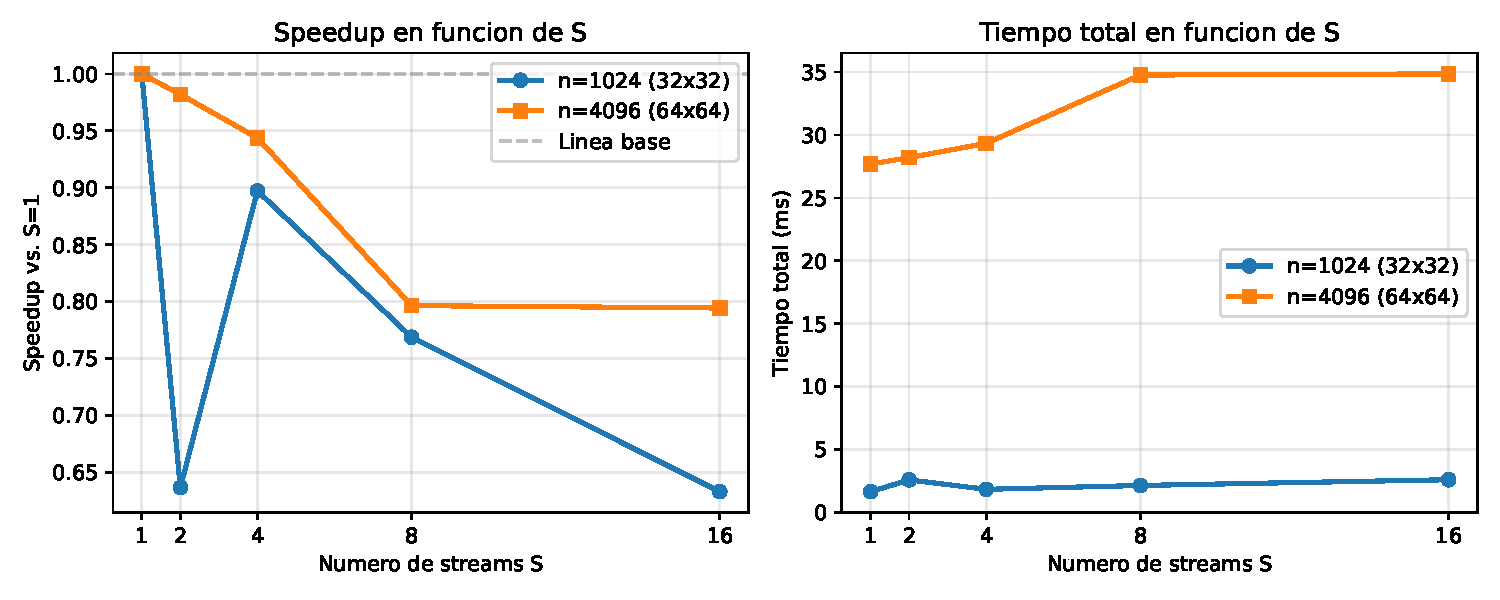
\includegraphics[width=0.8\textwidth]{speedup.pdf}
\caption{Speedup en función del número de streams $S$}
\end{figure}

%---------------------------------------------------------------------
\section{Análisis y discusión}
%---------------------------------------------------------------------

\subsection{Perfilado con Nsight Systems}

% Incluir diagrama/captura de Nsight Systems mostrando solapamiento

\subsection{¿A partir de cuántos streams el rendimiento deja de mejorar?}

\texttt{TODO: Discutir resultados empíricos vs. teóricos.}

\subsection{Limitación del bus PCIe}

\texttt{TODO: Analizar si la estrategia de latency hiding mitigó la limitación.}

\subsection{Viabilidad para datasets que superan la VRAM}

\texttt{TODO: Discutir escalabilidad y limitaciones de memoria.}

%---------------------------------------------------------------------
\section{Conclusiones}
%---------------------------------------------------------------------

\texttt{TODO}

%---------------------------------------------------------------------
\bibliographystyle{plain}
\begin{thebibliography}{9}

\bibitem{div2k}
E. Agustsson, R. Timofte,
\textit{DIV2K: DIVerse 2K Resolution Image Dataset},
\url{https://data.vision.ee.ethz.ch/cvl/DIV2K/}

\bibitem{cuda}
NVIDIA Corporation,
\textit{CUDA C++ Programming Guide},
\url{https://docs.nvidia.com/cuda/cuda-c-programming-guide/}

\bibitem{cimg}
D. Tschumperlé et al.,
\textit{The CImg Library},
\url{https://github.com/GreycLab/CImg}

\end{thebibliography}

\end{document}
